% LuaTeX Project Setup and Compilation Guide

% This document outlines the necessary steps to configure a comprehensive LaTeX environment
% for editing and typesetting documents using either Emacs with AUCTeX or the Kile editor.

%----------------------------------------------------------------------------------------
% Installing a TeX Distribution

% Choose one of the following TeX distributions based on your operating system:

% Linux:
%   TeX Live:*Recommended for its extensive package collection and regular updates.
%     ```bash
%     sudo dnf install texlive-full  % Comprehensive installation
%     sudo dnf install texlive-babel-russian  % Russian language support
%     ```
%   Other Distributions:*Explore options like TeX Live or TeXstudio depending on your preferences.
% Windows:
%   MiKTeX:*A popular choice with on-the-fly package installation. Download the installer from https://miktex.org/download.
% macOS:
%   MacTeX:*A complete TeX distribution specifically for macOS. Download from https://tug.org/mactex/.

%----------------------------------------------------------------------------------------
% Editor Configuration

% Select your preferred LaTeX editor:

% Doom Emacs
%   1. Install latex for doomemacs: Refer to the Emacs package manager or official instructions - https://docs.doomemacs.org/v21.12/modules/lang/latex/.
%   2. Optionally, install and configure `pdf-tools` for enhanced PDF interaction within Emacs.
% Kile:
%   1. Install Kile using your system's package manager or download from https://kile.org/.
%   2. Kile provides a user-friendly graphical interface with project management, syntax highlighting,
%      code completion, and integrated PDF viewing.

%----------------------------------------------------------------------------------------
% Compilation and Workflow

% Use the appropriate command or keybinding to compile your LaTeX document (e.g., `luatex` for PDF output).
% Configure your editor to automatically build and view the generated PDF.
% Utilize the features of your chosen editor and installed packages to enhance your LaTeX workflow.

%----------------------------------------------------------------------------------------
% Additional Resources

% Comprehensive TeX documentation: https://www.tug.org/texlive/doc.html
% LaTeX community forums and support: https://tex.stackexchange.com/
% Package documentation and examples: Refer to the respective package websites or CTAN (https://ctan.org/).

%----------------------------------------------------------------------------------------

% Useful resource - https://detexify.kirelabs.org/classify.html

\documentclass[14pt, a4paper]{extreport}

\usepackage[english, russian]{babel}
\usepackage{graphicx}
\usepackage[margin=2cm]{geometry} % Consistent margins
\usepackage{titlesec} % Customize section headings
\usepackage{fancyhdr} % Customize headers and footers
\usepackage{enumitem}
\usepackage{subfig}
\usepackage{hyperref}
\usepackage{authblk}
\usepackage{titling}
\usepackage[numbers]{natbib}
\usepackage{amsmath}
\usepackage{listings}
\usepackage{verbatim}
\usepackage{textcomp}
\usepackage{microtype} % best hyphen package

% \usepackage{texdoc} install this package for IDE quick documentation

\lstdefinestyle{bwstyle}{
    commentstyle=\itshape,
    keywordstyle=\bfseries,
    stringstyle=\ttfamily,
    basicstyle=\ttfamily\footnotesize,
    numbers=left,
    numberstyle=\tiny,
    stepnumber=1,
    numbersep=5pt,
    showspaces=false,
    showstringspaces=false,
    showtabs=false,
    tabsize=4,
    breaklines=true,
    breakatwhitespace=false,
    captionpos=b
}

\lstset{style=bwstyle, language=C++}
\lstset{style=bwstyle, language=python}


\hypersetup{
    colorlinks=false,
}

\title{МЕТОДЫ ОЦЕНКИ ВЛИЯНИЯ КОСМИЧЕСКОЙ ПОГОДЫ НА БОРТОВЫЕ СИСТЕМЫ НИЗКООРБИТАЛЬНЫХ СПУТНИКОВ}
\author{Глеба Е. М., Баранова В. С.}
\date{\today}

\graphicspath{{../img/}}

\babelfont{rm}
[Path=../fonts/,
    UprightFont=*-regular,
    BoldFont=*-bold,
    ItalicFont=*-italic,
    BoldItalicFont=*-bold-italic,
    Extension=.ttf
]{timesnrcyrmt}

\titleformat*{\section}{\Large\bfseries}
\titleformat*{\subsection}{\large\bfseries}

% Set up headers and footers
%\pagestyle{fancy}
%\fancyhf{} % Clear default headers and footers
%\fancyhead[C]{\textbf{Методы оценки влияния космической погоды}} % Centered header
%\fancyfoot[C]{\thepage} % Page number in footer

\renewcommand{\thesection}{\arabic{section}}

\titleformat{\subsection}[block]{\large\bfseries}{Глава \thesection.\thesubsection}{1em}{}

\begin{document}

    \setlength{\headheight}{14.0pt}

    \begin{titlepage}
        \begin{center}
            \textbf{МИНИСТЕРСТВО ОБРАЗОВАНИЯ РЕСПУБЛИКИ БЕЛАРУСЬ БЕЛОРУССКИЙ ГОСУДАРСТВЕННЫЙ УНИВЕРСИТЕТ ФАКУЛЬТЕТ РАДИОФИЗИКИ И КОМПЬЮТЕРНЫХ ТЕХНОЛОГИЙ
            } \\
            Кафедра физики и аэрокосмических технологий
        \end{center}

        \vspace{8em}

        \begin{center}
            \textbf{\thetitle}
        \end{center}
        
        \begin{center}
            {Курсовая работа}
        \end{center}

        \vspace{3cm}

        \hfill
        \parbox{17em}{
            Глеба Евгения Михайловича \newline
            обучающегося 3 курса специальности \newline
            «Аэрокосмические радиоэлектронные и информационные системы и технологии»

            \vspace{0.5cm}

            Научный руководитель: \newline
            Баранова Василина Сергеевна
        }

        \vspace{8cm}

        \begin{center}
            Минск, \the\year
        \end{center}

    \end{titlepage}

    \tableofcontents

    \newpage

    \section{Введение}

    Космическая погода представляет собой комплекс явлений, происходящих в околоземном космическом пространстве, которые могут влиять на работу низкоорбитальных спутников.
    К ним относятся: солнечные вспышки, выбросы корональной массы, геомагнитные бури.
    Влияние космической погоды может проявляться в виде аномалий телеметрии, сбоев в работе бортовых систем и даже полной потери спутника~\cite{green_2017_impact}.
    В большинстве случаев, для обнаружения аномалий используются критерии на основе пороговых значений нижних и верхних пределов наиболее критичных параметров телеметрии бортовой электроники наноспутника.
    Также в последнее время, в область проектирования и эксплуатации наноспутников внедряются автоматизированные системы мониторинга состояния телеметрии, которые используют различные модели машинного обучения\cite{schlag_2018_numerical}.
    Подобные автоматизированные системы оценивают в целом работоспособность бортовых систем на момент испытаний или в режиме полетной диагностики.
    Спутник является сложной электрической системой, где события на каждом узле (компоненты бортовых систем) могу привести к последовательности не предугаданных сбоев.
    Причиной сбоев может послужить как естественные неполадки бортовых компонентов, так и внешние факторы.
    В данной работе проводится оценка взаимосвязи и влияния солнечной активности на работу бортовой электроники по данным телеметрии космических аппаратов, а также разработка и оптимизация готовых решений с открытым исходным кодом для анализа больших данных.

    \newpage


    \section{SatNOGS: Открытая инфраструктура для мониторинга низкоорбитальных спутников}

    SatNOGS представляет собой комплексную платформу, обеспечивающую функционирование открытой сети наземных станций для мониторинга спутников.
    Основной целью проекта является разработка полного стека открытых технологий, основанных на открытых стандартах, и создание полноценной наземной станции в качестве демонстрации возможностей данного стека.
    Система SatNOGS способна принимать сигналы со спутников, находящихся на низкой околоземной орбите (LEO), в диапазонах UHF и VHF. Она позволяет извлекать сигналы состояния и телеметрии, данные с научных и исследовательских спутников (например, результаты магнитосферных экспериментов), метеорологические данные и другую информацию.

    \subsection{Ключевые элементы инфраструктуры}

    Проект SatNOGS зародился в 2014 году во время мероприятия NASA SpaceApps Hackathon, проходившего в Афинском хакерспейсе.
    Он предоставляет набор технологий, необходимых для создания распределенной сети наземных станций, предназначенных для наблюдения за спутниками на низкой околоземной орбите.
    Ключевыми компонентами SatNOGS являются:

    \begin{itemize}[label=\textbullet]
        \item    SatNOGS Network: Веб-приложение, предназначенное для планирования наблюдений по сети наземных станций.
        Оно способствует координации наблюдений за спутниковыми сигналами и планированию таких наблюдений среди наземных станций, подключенных к сети.
        \item    База данных SatNOGS: Ресурс, позволяющий пользователям предоставлять информацию о передатчиках активных спутников.
        Данные доступны через API или веб-интерфейс.
        \item    Клиент SatNOGS: Программное обеспечение, работающее на наземных станциях (обычно на встраиваемых системах).
        Оно получает регулярные задания на наблюдение из сети, принимает спутниковые передачи и отправляет их обратно в веб-приложение Network.
        \item    Наземная станция SatNOGS: Аппаратное обеспечение наземной станции с открытым исходным кодом, включающее ротаторы, антенны и электронику, подключенные к клиенту.
    \end{itemize}

    \subsection{Функционал и Применение}

    SatNOGS фокусируется на приеме данных со спутников, а не на отправке команд.
    Спутники обычно передают телеметрические данные практически непрерывно, что позволяет операторам и другим пользователям сети SatNOGS получать, декодировать и ретранслировать эту информацию.
    Одной из ключевых задач проекта является стимулирование разработчиков спутников (особенно создателей CubeSat) к использованию протоколов с открытым исходным кодом для передачи данных.
    Это обеспечивает дополнительную возможность декодирования таких протоколов системой SatNOGS и сбор телеметрической информации с множества различных наземных станций.

    \subsection{Преимущества проекта}

    SatNOGS реализует концепцию массового строительства и развертывания любительских станций слежения по всему миру, основанных на технологиях с открытым исходным кодом и открытых стандартах.
    Такой подход обеспечивает:

    \begin{itemize}[label=\textbullet]
        \item    Модульность: Система легко модифицируется и адаптируется к различным задачам.
        \item    Автономность: Станции подключаются к интернету и работают полностью автоматически.
        \item    Доступность: Открытый исходный код и стандарты способствуют широкому распространению и развитию технологий.
    \end{itemize}

    В целом, SatNOGS представляет собой мощный инструмент для мониторинга низкоорбитальных спутников, способствующий развитию открытой космической инфраструктуры.

    \subsection{SatNOGS NetWork}

    Для всех пользователей и гостей SatNOGS сеть предоставляет веб-интерфейс со всеми доступными наблюдениями и их соответствующие данные, которые представлены ниже.

    \begin{figure}[h!]
        \centering
        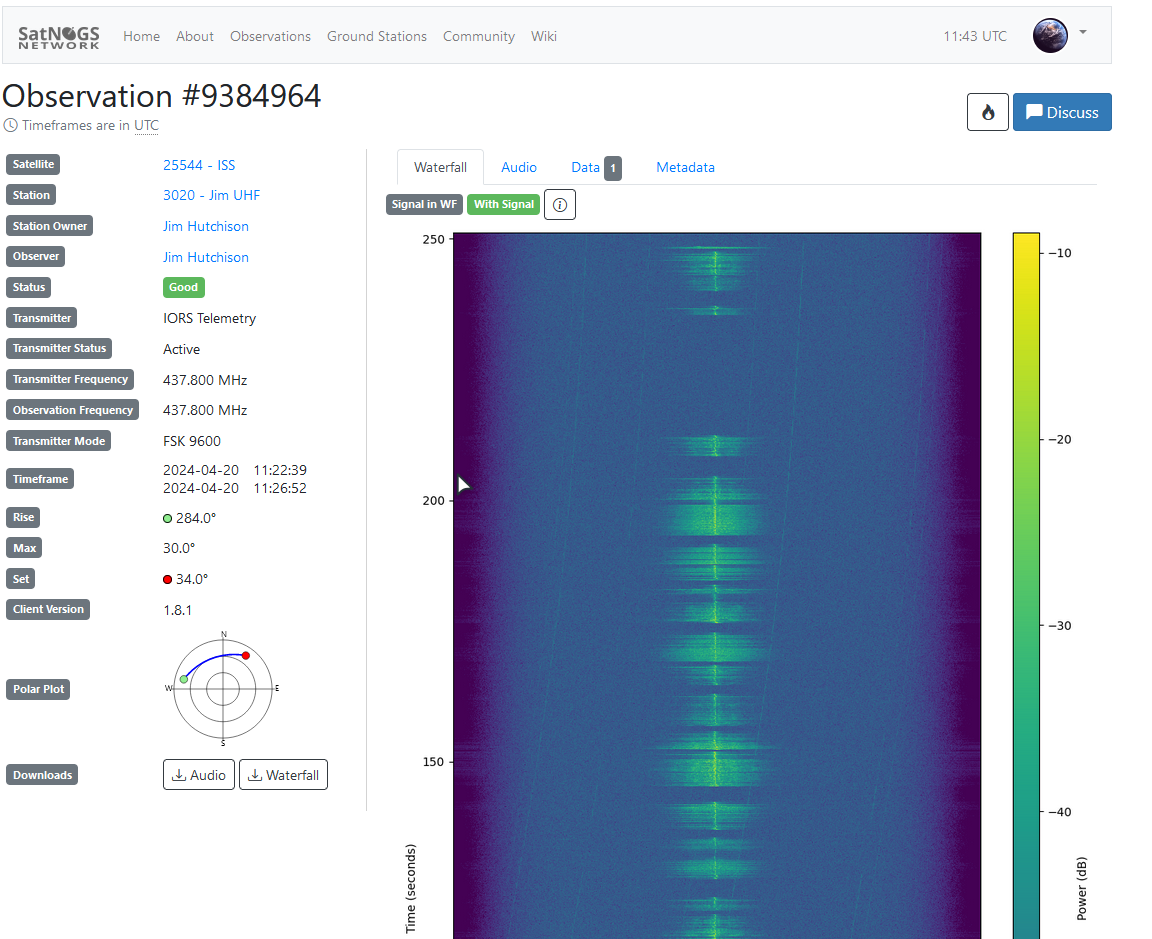
\includegraphics[width=0.8\textwidth]{satnogs_observation_example}
        \caption{Информация о наблюдениях и каскад сигнала}
        \label{fig:satnogs_observation_example}
    \end{figure}


    
    \begin{figure}[h!]
        \centering
        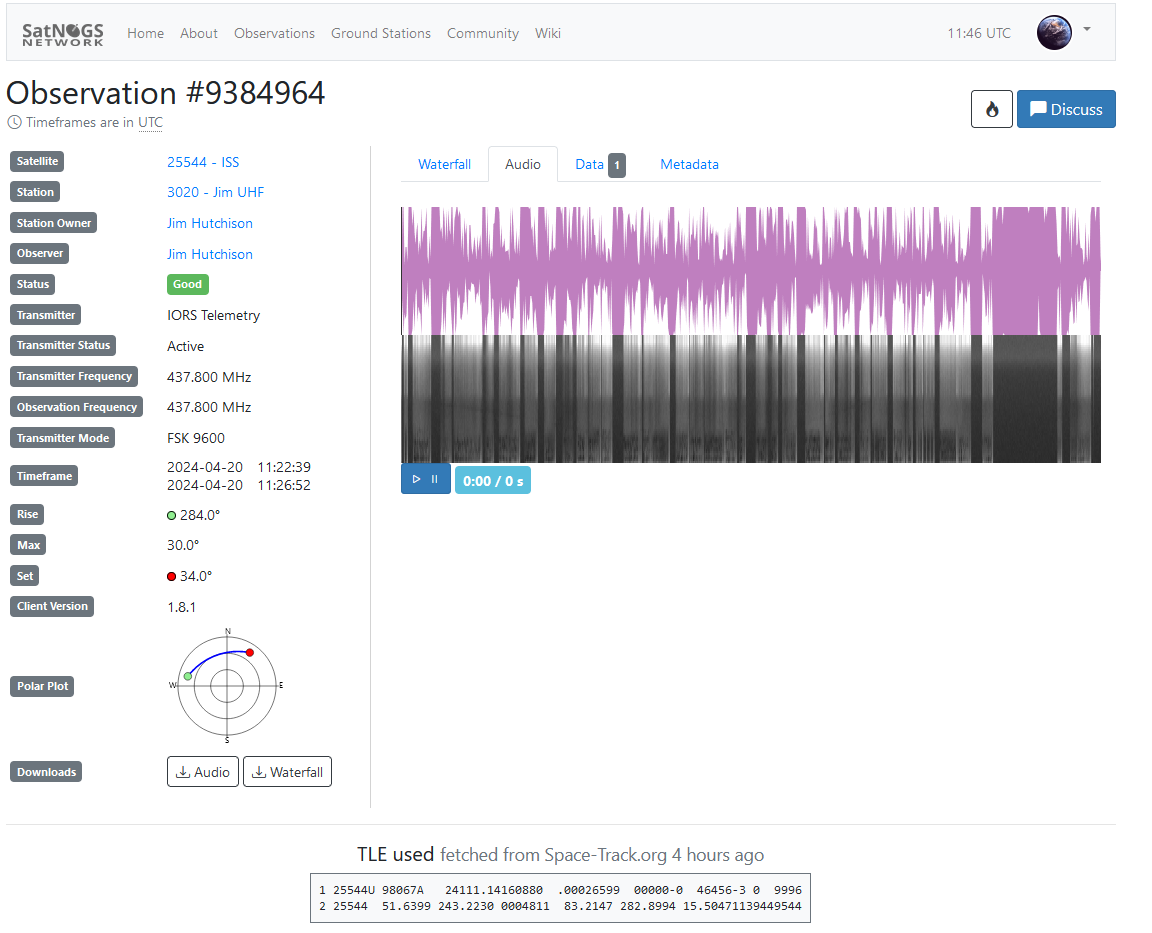
\includegraphics[width=0.8\textwidth]{satnogs_decoded_telemetry_example}
        \caption{Вкладка демодулированного аудиоплеера из наблюдения \#9384964}
        \label{fig:satnogs_decoded_telemetry_example}
    \end{figure}


    \begin{figure}[h!]
        \centering
        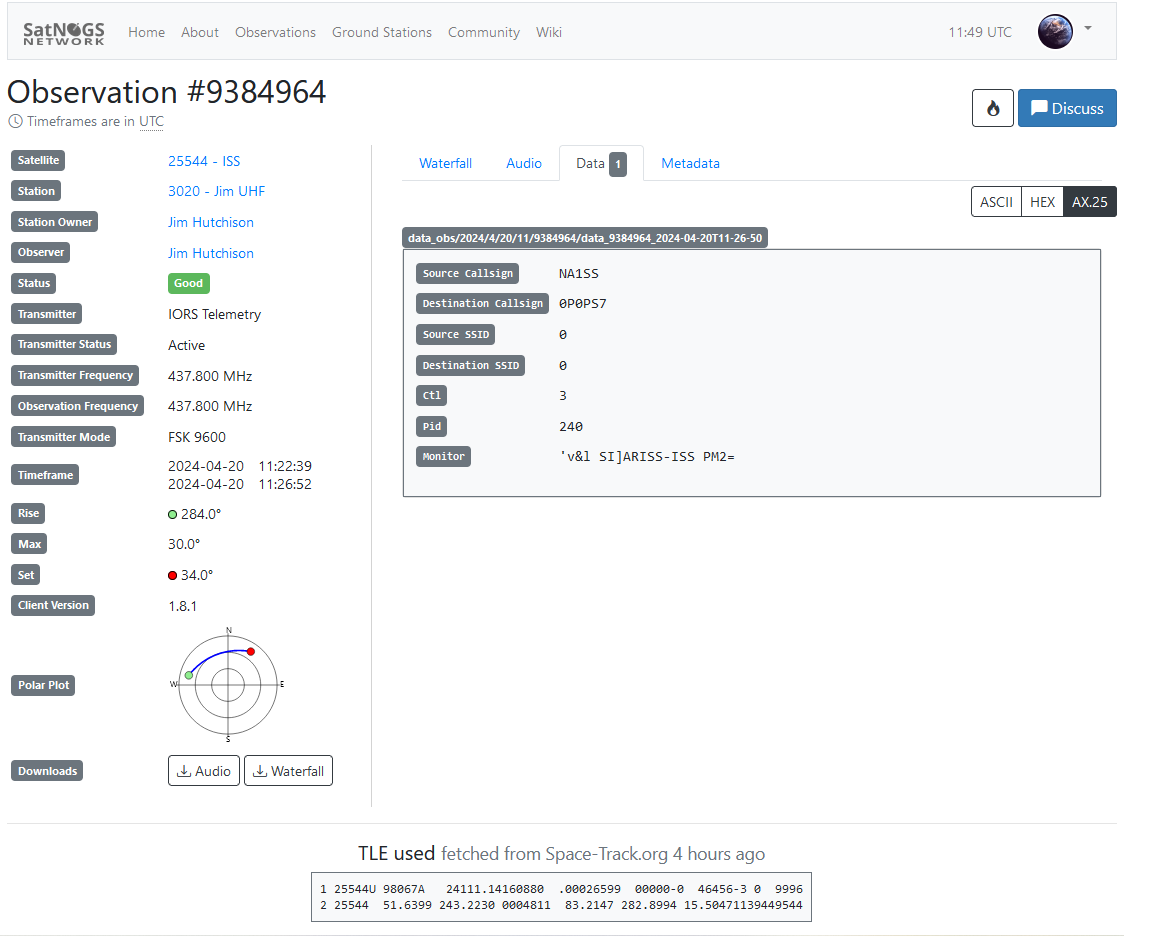
\includegraphics[width=0.8\textwidth]{satnogs_observation_data_example}
        \caption{Декодированные данные телеметрии DUV 25544 - ISS}
        \label{fig:satnogs_observation_data_example}
    \end{figure}

    \subsection{База данных SatNOGS: краеугольный камень распределенной сети наблюдений}

    Эффективное функционирование распределенной сети наблюдений за спутниками, как в проекте SatNOGS, требует централизованного и актуального источника информации о космических аппаратах.
    База данных SatNOGS призвана восполнить пробел в доступности подобной информации, предоставляя открытый и постоянно обновляемый ресурс для всего сообщества.

    \subsubsection{Содержание и структура}

    База данных SatNOGS хранит обширный набор данных о каждом космическом аппарате на орбите Земли, включая:

    \begin{itemize}
        \item \textbf{Орбитальные параметры:} База данных содержит кеплеровы элементы орбиты каждого спутника,  математические параметры, позволяющие с высокой точностью рассчитать и предсказать положение спутника в любой момент времени.
        \item \textbf{Телекоммуникационные характеристики:} Хранит информацию о частотах, используемых спутником для передачи данных,  режимах модуляции сигнала и протоколах передачи данных, необходимых для настройки оборудования наземной станции и корректного приема информации.
        \item \textbf{Телеметрические данные:}  База данных накапливает декодированные кадры телеметрии, полученные с наземных станций сети SatNOGS. Эти данные предоставляют ценную информацию о состоянии бортовых систем спутника, его работе и научных измерениях.
    \end{itemize}

    \subsubsection{Краудсорсинг и открытость}

    Ключевым принципом базы данных SatNOGS является краудсорсинг.
    Пользователи и операторы наземных станций могут вносить свой вклад, предоставляя информацию о новых спутниках, обновляя существующие данные или делясь телеметрическими кадрами.
    Все изменения проходят модерацию и становятся доступными для всей сети.

    Взаимодействие с базой данных осуществляется через веб-интерфейс и открытый API, что позволяет легко интегрировать ее с другими приложениями и системами.

    \subsubsection{Идентификация и извлечение данных}

    Спутники в базе данных идентифицируются по номеру каталога космических объектов NORAD (USSPACECOM) и общепринятому имени.
    Для каждого объекта хранится набор записей о транспондерах, включая частоты и форматы модуляции.
    Эта информация используется сетью SatNOGS для расчета видимости спутников и планирования наблюдений.

    \subsubsection{Взаимодействие с клиентом SatNOGS}

    Клиент SatNOGS, программное обеспечение, управляющее наземной станцией, активно взаимодействует с базой данных:

    \begin{itemize}
        \item \textbf{Получение данных о наблюдениях:} Клиент запрашивает у базы данных информацию о видимых в данный момент спутниках и их параметрах передачи данных (частоты, модуляция и т.д.).
        \item \textbf{Отправка телеметрии:} После успешного приема и демодуляции сигнала со спутника, клиент отправляет декодированные кадры телеметрии в базу данных для хранения и дальнейшего анализа.
        \item \textbf{Отчетность:} Клиент SatNOGS передает в базу данных журналы работы, содержащие информацию о выполненных операциях,  и другие отчеты о состоянии наземной станции, включая информацию о работоспособности оборудования и возможных ошибках.
    \end{itemize}

    \begin{figure}[h!]
        \centering
        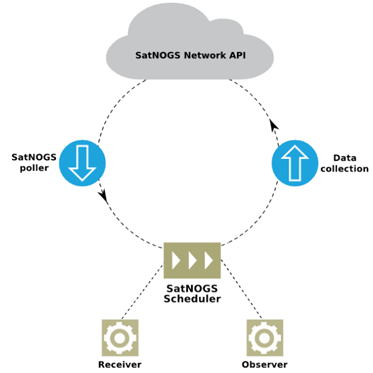
\includegraphics[width=0.5\textwidth]{satnogs_client_program_interactions}
        \caption{Клиентские программные компоненты и взаимодействия с базой данных SatNOGS.}
        \label{fig:satnogs_client_program_interactions}
    \end{figure}

    \subsubsection{Значение для сети SatNOGS}

    База данных SatNOGS играет ключевую роль в успешной работе распределенной сети наблюдений:

    \begin{itemize}
        \item \textbf{Обеспечение актуальной информацией:} База данных SatNOGS предоставляет наземным станциям актуальную информацию о орбитальных параметрах и телекоммуникационных характеристиках спутников, что позволяет эффективно планировать наблюдения и принимать сигналы.
        \item \textbf{Содействие сотрудничеству:} Открытый характер базы данных и возможность совместного внесения данных способствует сотрудничеству между участниками сообщества SatNOGS, объединяя их усилия для сбора и анализа данных о космических аппаратах.
        \item \textbf{Открытость и доступность:} Свободный доступ к информации о спутниках, хранящейся в базе данных SatNOGS, делает ее ценным ресурсом для исследователей, студентов и всех, кто интересуется космической тематикой, способствуя развитию научных и образовательных проектов.
    \end{itemize}

    База данных SatNOGS является ярким примером того, как открытость, краудсорсинг и современные технологии могут быть использованы для создания мощного инструмента для изучения космоса.

    \subsection{Визуализация данных телеметрии: хранилище данных и Kaitai Struct}

    Сбор и хранение данных телеметрии со спутников - важная задача, но не менее важно предоставить инструменты для их анализа и интерпретации.
    Хранилище данных SatNOGS в сочетании с платформой Kaitai Struct предлагает эффективное решение для визуализации и изучения данных телеметрии, делая их доступными и понятными для инженеров и исследователей.

    \subsubsection{Kaitai Struct: декларативное описание двоичных данных}

    Kaitai Struct - это мощный инструмент с открытым исходным кодом, предназначенный для описания структуры двоичных данных с помощью декларативного языка.
    Это позволяет создавать формализованные спецификации форматов данных,  независимые от конкретного языка программирования или платформы.

    \subsubsection{Применение Kaitai Struct в SatNOGS}

    \begin{enumerate}
        \item \textbf{Описание формата данных:} Для каждого типа спутника или используемого формата телеметрии создается файл описания структуры данных с расширением ``.ksy`` на языке Kaitai Struct.
        Этот файл содержит формализованное описание того, как байты в потоке данных должны интерпретироваться и преобразовываться в значимые значения (например, числа, строки, структуры данных).
        \item \textbf{Обработка данных:} Кадры данных телеметрии, извлеченные из базы данных SatNOGS~\cite{satnogs_database_docs}, обрабатываются с использованием соответствующего файла описания Kaitai Struct.
        Программа-парсер Kaitai Struct использует это описание для разбора двоичных данных и извлечения значений согласно заданной структуре.
        \item \textbf{Визуализация:} Полученные после обработки данные преобразуются в формат, совместимый с платформой Grafana~\cite{satnogs_grafana_docs}.
        Grafana позволяет создавать информативные и наглядные визуализации данных в виде графиков, диаграмм, таблиц и других элементов,  что облегчает анализ и интерпретацию телеметрии.
    \end{enumerate}

    \subsubsection{Преимущества подхода}

    \begin{itemize}[label={--}]
        \item \textbf{Универсальность:} Kaitai Struct поддерживает генерацию кода для множества языков программирования, таких как Python, Java, C++ и другие.
        Это обеспечивает легкую интеграцию с различными системами и инструментами обработки данных.
        \item \textbf{Читабельность:}  Декларативный язык Kaitai Struct позволяет описывать структуру данных в понятной и легко читаемой форме,  близкой к естественному языку.
        Это упрощает понимание формата данных и поддержку файлов описания.
        \item \textbf{Гибкость:} Grafana предоставляет широкий набор инструментов для визуализации данных, включая различные типы графиков, диаграмм, таблиц и интерактивных элементов.
        Это позволяет адаптировать представление информации под конкретные задачи и потребности пользователей.
    \end{itemize}

    \subsubsection{Заключение}

    Использование Kaitai Struct и Grafana в хранилище данных SatNOGS значительно упрощает анализ и интерпретацию данных телеметрии, предоставляя инженерам и исследователям удобный инструмент для изучения работы спутников и получаемой с них научной информации.

    \subsection{Текущее состояние сети SatNOGS: от скромных начинаний к глобальной инфраструктуре}

    С момента своего запуска в 2015 году сеть SatNOGS прошла путь от нескольких экспериментальных наземных станций до разветвленной глобальной инфраструктуры, обслуживающей тысячи наблюдений за спутниками ежедневно.

    \subsubsection{Экспоненциальный рост и развитие}

    \begin{itemize}
        \item \textbf{Увеличение количества наземных станций:} Растущий интерес к малым спутникам CubeSat и открытость платформы SatNOGS привели к экспоненциальному росту числа зарегистрированных и активных наземных станций в сети.
        \item \textbf{Расширение функциональности:}  Постоянное развитие экосистемы SatNOGS, включая внедрение таких функций, как автоматическое декодирование телеметрии и визуальный анализ спектра,  значительно повысило ценность проекта и предоставляемых им данных.
    \end{itemize}

    \subsubsection{Статистика наблюдений}

    \begin{itemize}
        \item \textbf{Количество наблюдений:} Сеть SatNOGS в настоящее время проводит около 1200 наблюдений за спутниками в день, что демонстрирует значительный рост по сравнению с несколькими десятками наблюдений в день на ранних этапах проекта в 2015 году.
        \item \textbf{Качество данных:} Примерно 70\% проводимых наблюдений содержат полезную информацию и телеметрию.
        Остальные наблюдения классифицируются как ``плохие`` (содержащие помехи или неполные данные) или``неудачные`` (не удалось загрузить данные из-за технических проблем).
        \item \textbf{Объем телеметрии:}  База данных SatNOGS ежедневно пополняется значительным объемом данных: около 2500 декодированных кадров телеметрии, полученных с различных спутников,  добавляются в хранилище.
    \end{itemize}

    \subsubsection{Ключевые принципы и цели}

    \begin{itemize}
        \item \textbf{Открытость и доступность:} Проект SatNOGS придерживается философии открытого программного и аппаратного обеспечения, делая технологии наблюдения за спутниками доступными для всех желающих, независимо от их опыта и ресурсов.
        \item \textbf{Сотрудничество и сообщество:} SatNOGS объединяет сообщество радиолюбителей, инженеров, исследователей и энтузиастов космоса, предоставляя платформу для совместной работы, обмена знаниями и опытом,  а также совместного развития проекта.
        \item \textbf{Дальнейшее развитие:} Планы развития SatNOGS включают в себя:
        \begin{itemize}
            \item Автоматизацию системы проверки данных с использованием методов машинного обучения для повышения эффективности и точности анализа.
            \item Оптимизацию планирования наблюдений для максимального использования ресурсов сети и обеспечения наилучшего качества данных.
            \item Расширение возможностей анализа данных, включая предоставление необработанных данных с радиоприемников для использования в радиоастрономических и других научных исследованиях.
        \end{itemize}
    \end{itemize}

    \subsubsection{Значение для сообщества}

    SatNOGS предоставляет широкий спектр инструментов и возможностей для изучения космоса~\cite{satnogs_general_docs},  включая:

    \begin{itemize}
        \item \textbf{Получение данных с CubeSat и других спутников:} SatNOGS предоставляет инструменты и инфраструктуру для приема и декодирования данных с малых спутников формата CubeSat, а также с других низкоорбитальных спутников,  открывая возможности для исследований и образовательных проектов.
        \item \textbf{Развитие навыков в области радиотехники и обработки сигналов:} Участие в проекте SatNOGS позволяет развивать практические навыки в области радиотехники, обработки сигналов, работы с радиолюбительским оборудованием и программным обеспечением.
        \item \textbf{Участие в научных и образовательных проектах:} SatNOGS активно поддерживает использование сети для научных исследований и образовательных проектов, предоставляя доступ к данным и инструментам для анализа.
        \item \textbf{Содействие развитию открытых космических технологий:} Проект SatNOGS способствует продвижению и развитию открытых космических технологий, делая исследования космоса более доступными и демократичными.
    \end{itemize}

    \newpage


    \section{Платформа Polaris ML}

    Приложение Polaris ML от LibreSpace~\cite{librespace_docs} использует алгоритм машинного обучения XGBoost для анализа взаимосвязей между параметрами телеметрии бортовых систем спутника~\cite{ray_2002_bayesian}.
    Polaris ML способен рассчитать и визуализировать взаимосвязи между параметрами телеметрии и степень их влияния друг на друга в виде трехмерного графа связностей.
    В процессе исследования производительность модели искусственного интеллекта Polaris ML была значительно усовершенствована путем переноса core инфраструктуры на C++, а именно выделением прекомпилированных библиотек ввода/вывода и кэширования промежуточных расчетов обучения.
    Также в приложение Polaris были добавлены декодеры для отслеживания целевых спутников и модуль, собирающий информацию о солнечной активности, работающий в отдельном контейнере Docker.
    Кроме того, был доработан инструмент для построения графов связностей и веб-интерфейс.
    Внедрены решения для прямого взаимодействия с панелью управления сервера SatNOGS, что позволяет получать дополнительные данные о состоянии интересующих спутников.
    На рис. \ref{fig:polaris_architecture} представлена архитектура финальной системы, включающая в себя внесенные доработки и усовершенствования.

    \begin{figure}[htbp]
        \centering
        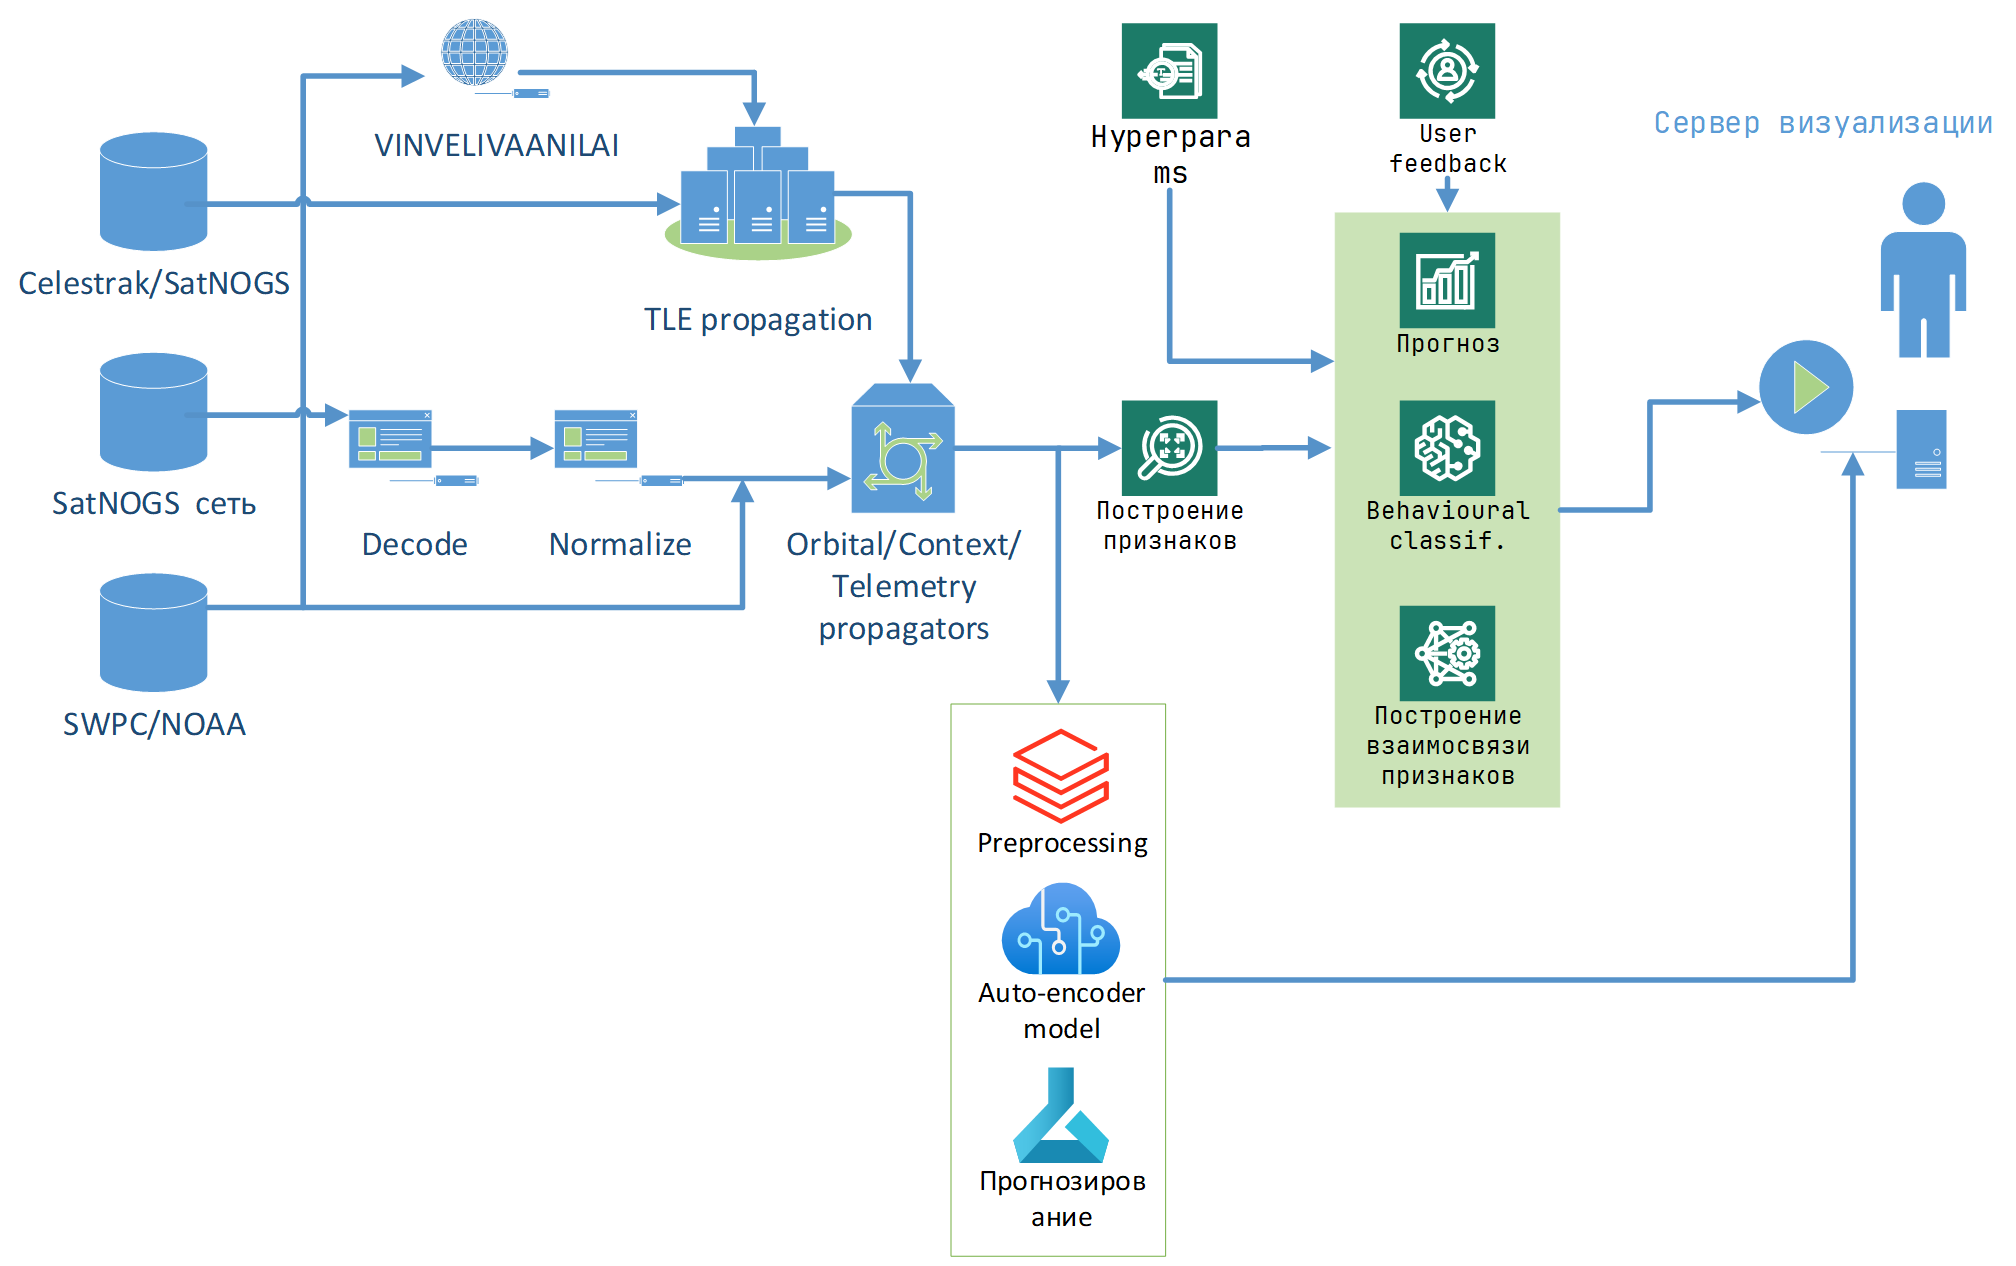
\includegraphics[width=0.8\textwidth]{polaris_architecture}
        \caption{Архитектура приложения Polaris}
        \label{fig:polaris_architecture}
    \end{figure}

    Система Polaris ML построена по модульному принципу, что обеспечивает гибкость и масштабируемость решения (см. Рис. \ref{fig:polaris_architecture}).

    \textbf{Модуль сбора и предобработки данных.} Данный модуль отвечает за получение телеметрической информации с целевых спутников.
    Интеграция с панелью управления SatNOGS позволяет получать доступ к широкому спектру данных, включая:
    \begin{itemize}
        \item \textbf{Параметры орбиты:} высота, наклонение, период обращения и др.
        \item \textbf{Данные о состоянии бортовых систем:} напряжение, ток, температура и др.
        \item \textbf{Информация о научных приборах.}
    \end{itemize}

    Полученные данные проходят предварительную обработку: очистку от шумов, заполнение пропусков, нормализацию и другие преобразования, необходимые для корректной работы алгоритмов машинного обучения.

    \textbf{Модуль анализа данных на основе XGBoost.} Ядром системы Polaris ML является алгоритм XGBoost (Extreme Gradient Boosting), представляющий собой ансамблевый метод машинного обучения, основанный на градиентном бустинге.
    XGBoost обладает рядом преимуществ, делающих его оптимальным выбором для анализа телеметрии спутников:

    \begin{itemize}
        \item \textbf{Высокая точность предсказаний:} XGBoost способен выявлять сложные нелинейные зависимости в данных, что позволяет строить высокоточные модели~\cite{behaviour_based_anomaly_detection}.
        \item \textbf{Устойчивость к переобучению:} алгоритм включает в себя механизмы регуляризации, предотвращающие переобучение модели на тренировочных данных.
        \item \textbf{Эффективность работы с большими объемами данных:} XGBoost хорошо масштабируется и может обрабатывать большие объемы данных за приемлемое время.
        \item \textbf{Модуль визуализации.} Для удобства интерпретации результатов анализа Polaris ML предоставляет возможность визуализации взаимосвязей между параметрами телеметрии в виде трехмерного графа связностей.
        \item \textbf{Оптимизация Производительности.} Важным этапом разработки Polaris ML стала оптимизация производительности системы.
    \end{itemize}

    Этапы проведения анализа:

    \begin{enumerate}[label=\arabic*.]
        \item \textbf{Автоматическое извлечение данных:}
        Данные извлекаются из различных источников, включая телеметрию сети SatNOGS и данные о космической погоде от NASA SWPC (NOAA).

        \item \textbf{Машинное обучение (XGBoost):}
        С использованием алгоритма XGBoost~\cite{xgboost_docs,boumghar_2018_enhanced} анализируется взаимосвязь извлеченных данных.
        Результатом является файл в формате JSON, содержащий описания параметров телеметрии и их значения в кадрах с временными метками.

        \item \textbf{Визуализация:}
        Строится граф связности для визуализации взаимозависимостей между параметрами.
        Также создается сложенный нормализованный вид телеметрии для отображения аномалий.

        \item \textbf{Экспорт данных:}
        Выходные данные графиков экспортируются для дальнейшего анализа и интерпретации.
    \end{enumerate}

    Как упоминалось ранее, был создан дополнительный модуль, который извлекает информацию о космической погоде с серверов NASA SWPC/NOAA. Эти данные сохраняются в базу данных InfluxDB, которая развернута локально в отдельном контейнере Docker Compose.
    Модуль также оснащен функциями для анализа данных орбитальных параметров в форматах TLE и OMM, а также для прогнозирования движения спутников на основе этих данных~\cite{bottou_1991_stochastic,killick_2012_optimal}.

    \subsection{Алгоритм XGBoost}

    \begin{enumerate}[label=\arabic*.]
        \item \textbf{Инициализация модели:}
        Определяется начальная модель $F_0(x)$ как константа, минимизирующая функцию потерь на обучающей выборке:

        \[F_0(x) = \arg \min_{\gamma} \sum_{i=1}^n L(y_i, \gamma)\]

        \item \textbf{Итеративное построение ансамбля:}
        Процесс построения модели происходит итеративно, добавляя по одному дереву за раз:
        \begin{enumerate}[label=\roman*.]
            \item \textbf{Вычисление градиентов и значений функции потерь:} Для каждого объекта в обучающей выборке вычисляются градиент ($g_i$) и значение функции потерь ($h_i$):

            \begin{gather*}
                g_i = \frac{\partial L(y_i, F_{m-1}(x_i))}{\partial F_{m-1}(x_i)}\\
                h_i = \frac{\partial^2 L(y_i, F_{m-1}(x_i))}{\partial F_{m-1}(x_i)^2}\\
            \end{gather*}

            \item \textbf{Построение дерева решений:} Строится дерево решений $f_m(x)$, минимизирующее функцию потерь с учетом регуляризации:

            \[\mathcal{L}^{(m)} = \sum_{i=1}^n \left[ g_i f_m(x_i) + \frac{1}{2} h_i f_m^2(x_i) \right] + \Omega(f_m)\]

            где $\Omega(f_m)$ - функция регуляризации, контролирующая сложность дерева.

            \item \textbf{Обновление модели:} Модель обновляется путем добавления нового дерева с весом, определяемым коэффициентом обучения $\alpha_m$:

            \[F_m(x) = F_{m-1}(x) + \alpha_m f_m(x)\]
        \end{enumerate}

        \item \textbf{Предсказание:}
        Для нового объекта $x$ предсказание модели получается суммированием предсказаний всех деревьев:

        \[\hat{y} = F_M(x) = \sum_{m=1}^M \alpha_m f_m(x)\]
    \end{enumerate}

    Особенности XGBoost:

    \begin{itemize}
        \item \textbf{Регуляризация:} Предотвращает переобучение и повышает обобщающую способность модели.
        \item \textbf{Метод Ньютона-Рафсона:} Используется для эффективной оптимизации функции потерь.
        \item \textbf{Обработка разреженных данных:} XGBoost эффективно работает с разреженными данными, что важно для многих задач.
        \item \textbf{Параллельное вычисление:} Алгоритм поддерживает параллельное вычисление для ускорения обучения, что и было полноценно добавлено в рамках данной курсовой работы.
    \end{itemize}

    \subsection{Процесс анализа}

    \begin{enumerate}[label=\arabic*.]
        \item \textbf{Извлечение фреймов:} Процесс анализа начинается с сегментации временного ряда телеметрии на фреймы.
        Это может быть выполнено с фиксированным размером окна или на основе определенных событий.
        \item \textbf{Извлечение признаков:} Из каждого фрейма извлекаются разнообразные статистические характеристики, такие как среднее значение, стандартное отклонение, минимум, максимум и другие, формируя вектор признаков.
        \item \textbf{Обучение модели XGBoost:} Модель XGBoost обучается на основе векторов признаков, полученных из фреймов.
        Цель - создать модель, способную предсказывать значения параметров телеметрии в будущих фреймах.
        \item \textbf{Выявление аномалий:} Аномалии определяются как значительные отклонения от предсказанных моделью XGBoost значений.
        Для этого Polaris ML предлагает несколько подходов:
        \begin{enumerate}[label=\alph*.]
            \item \textbf{Пороговые значения:} Устанавливаются пределы отклонений от предсказанных значений, например:

            \[\| y_i - \hat{y}_i \| > \epsilon\]

            где $y_i$ - реальное значение, $\hat{y}_i$ — предсказанное значение, а $\epsilon$ - заданный порог.
            \item \textbf{Статистические методы:} Используются z-оценка:

            \[z_i = \frac{y_i - \mu}{\sigma}\]

            где $\mu$ - среднее значение, $\sigma$ — стандартное отклонение, и тест Граббса:

            \[G = \frac{\max_{i}|y_i - \bar{y}|}{s}\]

            где $\bar{y}$ - выборочное среднее, $s$ - выборочное стандартное отклонение, для выявления выбросов.
        \end{enumerate}
        \item \textbf{Графы связности:} Модель XGBoost также используется для построения графов связности, визуализирующих взаимосвязи между параметрами телеметрии.
        Это помогает анализировать влияние изменений одних параметров на другие и выявлять потенциальные причины аномалий.
    \end{enumerate}

    \subsection{Улучшение ядра XGBoost}

    В рамках курсовой работы была проведена оптимизация алгоритма градиентного бустинга XGBoost с использованием NVIDIA CUDA и Tensor Cores.

    \subsubsection{Использование CUDA и Shared Memory}

    Для ускорения вычислений на GPU, был реализован kernel, использующий CUDA для параллельной обработки данных.
    В частности, в алгоритме предсказания листьев деревьев, был использован shared memory для повышения эффективности доступа к данным, см. приложение~\ref{subsec:xgboost_cuda_shared_memory_upgrade}.
    Shared memory \textemdash{} это высокоскоростная память, доступная всем ядрам потоковой мультипроцессорной системы (SM) на GPU\@.

    \begin{itemize}
        \item Kernel PredictLeafKernelSharedMem использует shared memory для хранения данных\@.
        \item Доступ к shared memory осуществляется быстрее, чем к глобальной памяти GPU\@.
        \item Такой подход позволяет значительно ускорить вычисления в алгоритме предсказания листьев\@.
    \end{itemize}

    \subsubsection{Использование Tensor Cores}

    Tensor Cores – это специализированные вычислительные блоки на GPU, оптимизированные для выполнения операций с матрицами.
    Для использования Tensor Cores, необходимо выполнить определенные требования к выравниванию памяти и размеру матриц ~\ref{subsec:xgboost_cuda_tensor_upgrade}.
    \begin{itemize}
        \item Kernel PredictLeafKernelTensorCore использует библиотеку cuBLAS для выполнения операций с матрицами.
        \item Выполнение операции матричного умножения с помощью cuBLAS позволяет эффективно использовать Tensor Cores.
        \item Исходные данные должны быть выровнены по границе 16 байт для оптимизации производительности Tensor Cores.
        \item Данные копируются в глобальную память GPU, после чего вычисляется матричное умножение с помощью cuBLAS\@.
        \item Результаты умножения возвращаются в глобальную память, а затем используются в алгоритме предсказания листьев.
    \end{itemize}

    Начиная с версии cuBLAS 11.0.0, больше нет ограничений на размеры матрицы и выравнивание памяти для использования тензорных ядер~\cite{nvidia_cublas_docs}.
    Однако наилучшая производительность при использовании тензорных ядер может быть достигнута, если размеры матрицы и указатели соответствуют определенным требованиям к выравниванию памяти.
    В частности, для получения максимальной производительности тензорных ядер должны быть выполнены все следующие условия:

    \begin{itemize}
        \item \texttt{m \% 8 == 0}
        \item \texttt{k \% 8 == 0}
        \item \texttt{op\_B == CUBLAS\_OP\_N || n \% 8 == 0}
        \item \texttt{intptr\_t(A) \% 16 == 0}
        \item \texttt{intptr\_t(B) \% 16 == 0}
        \item \texttt{intptr\_t(C) \% 16 == 0}
        \item \texttt{intptr\_t(A + lda) \% 16 == 0}
        \item \texttt{intptr\_t(B + ldb) \% 16 == 0}
        \item \texttt{intptr\_t(C + ldc) \% 16 == 0}
    \end{itemize}

    Для выполнения вышеперечисленных условий был изменен механизм разбивания блоков нормализованных данных для их последующего анализа.
    Таким образом, полученный pipeline для обработки извлеченных данных нейросетевым ансамблем XgBoost представлен на рис.~\ref{fig:polaris_xgboost_pipeline}.

    \begin{figure}[!htbp]
        \centering
        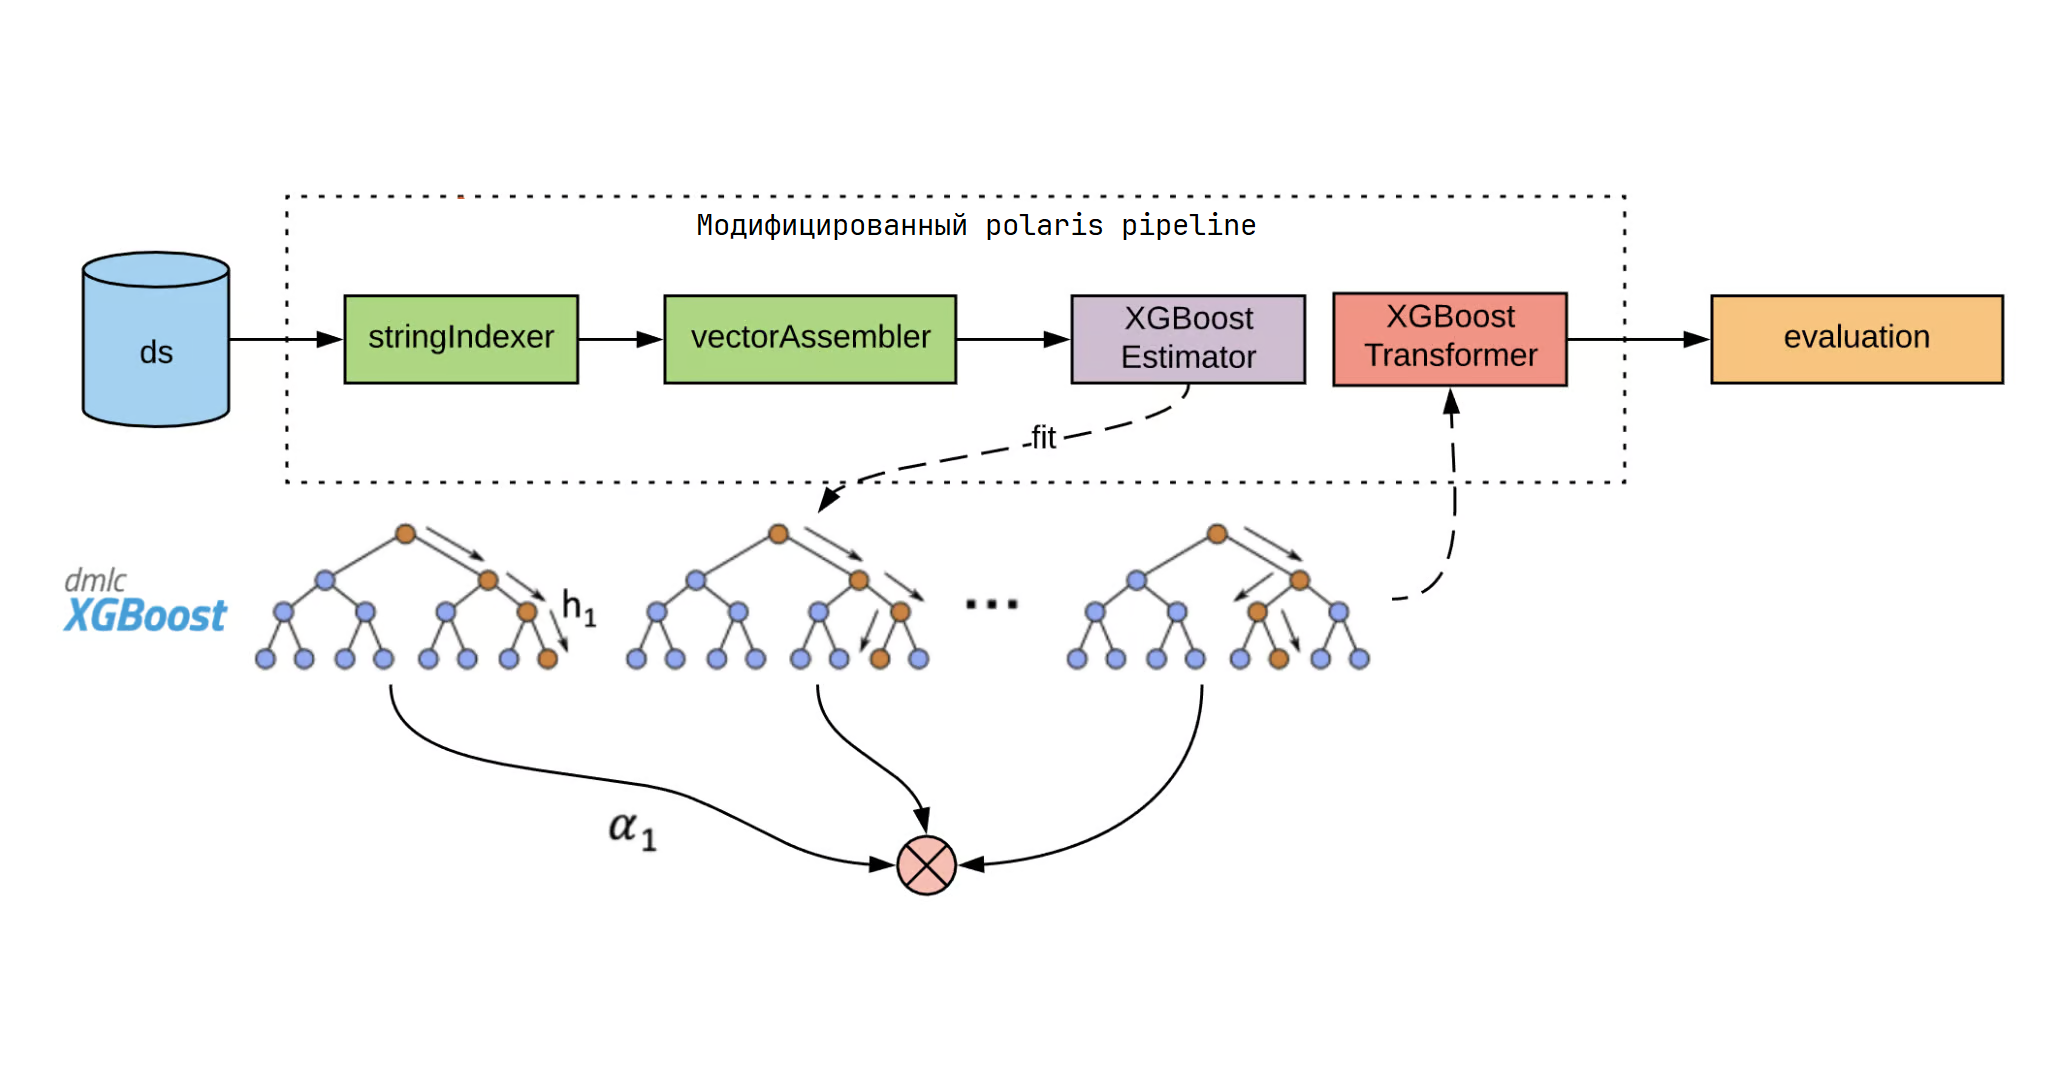
\includegraphics[width=1.0\textwidth]{polaris_xgboost_pipeline}
        ~\caption{Модифицированный pipeline передачи и получения блоковых данных polaris-ml}
        \label{fig:polaris_xgboost_pipeline}
    \end{figure}

    Этапы преобразования и обучения в обзем и целом остались неизменными.
    На этапе преобразования объектов мы обычно выполняем однократное кодирование или используем нашу внутреннюю реализацию пакетного StringIndexer для преобразования категориальных столбцов в индексированные столбцы перед выполнением последовательности преобразований объектов и этапов условного вычисления.
    Затем преобразованные объекты передаются в XGBoost trainer.
    Платформа оценки загружает сгенерированную модель и функции XGBoost для вычисления важности функций и настраиваемых показателей производительности модели, указанных пользователем.
    Все вышеперечисленное представлено на рис.~\ref{fig:xgboost_processing}.

    \begin{figure}[!htbp]
        \centering
        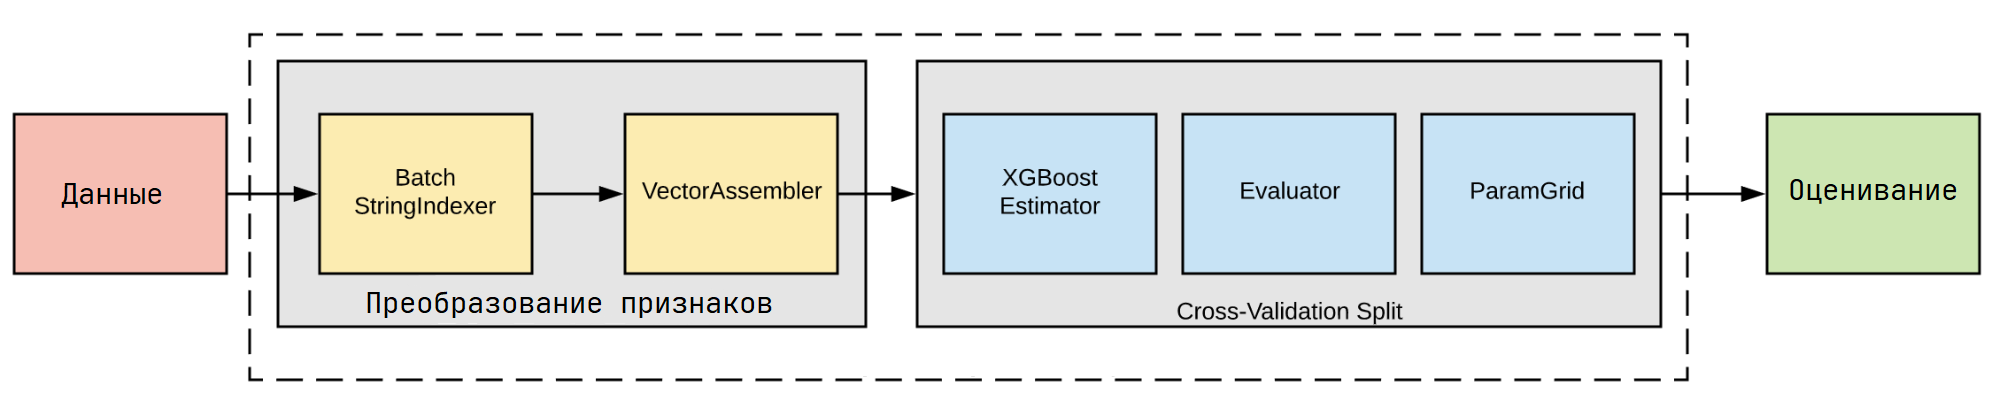
\includegraphics[width=1.0\textwidth]{xgboost_processing}
        ~\caption{Рабочий процесс обучения в XGBoost состоит из двух этапов, которые очищают и обрабатывают необработанные данные для использования при оценке модели ML.}
        \label{fig:xgboost_processing}
    \end{figure}

    \section{Анализ перезагрузок основного процессор и граф связности}

    На рис.\ref{fig:grifex_resets_vs_solar_params} представлена взаимосвязь количества перезагрузок основного процессора наноспутника формата 3U GRIFEX от следующих индексов солнечной активности за период с 2019-03-03 по 2024-02-22: среднемесячные значения пятен S.I.D.C., SWPC/SWO и f10.7 см радиоизлучение.
    На рис.\ref{fig:grifex_graph} представлен результат использования модели Polaris ML для построения 3D графа связности параметров телеметрии спутника GRIFEX за период 2015–2022 г.
    Все точечные диграммы построены кодом из приложения~\ref{subsec:dot_diagram_code}.

    \begin{figure}[htbp]
        \centering
        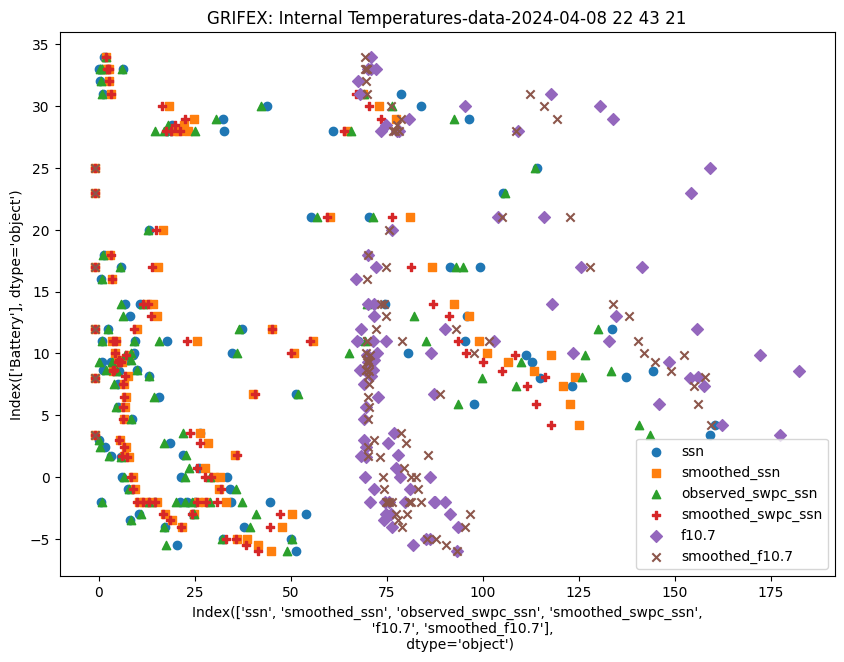
\includegraphics[width=1.0\textwidth]{grifex_battery_vs_solar}
        ~\caption{Точечная диаграмма внутренних температур с набором параметров солнечной активности}
        \label{fig:grifex_battery_vs_solar}
    \end{figure}

    \begin{figure}[htbp]
        \centering
        \subfloat[]{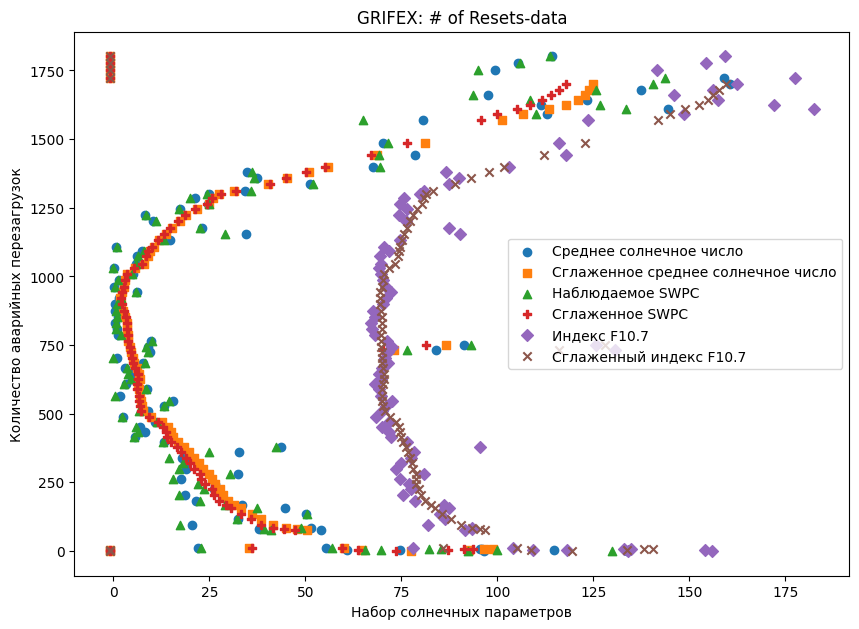
\includegraphics[width=0.80\textwidth]{grifex_resets_vs_solar_params}\label{fig:grifex_resets_vs_solar_params}}
        \hfill
        \subfloat[]{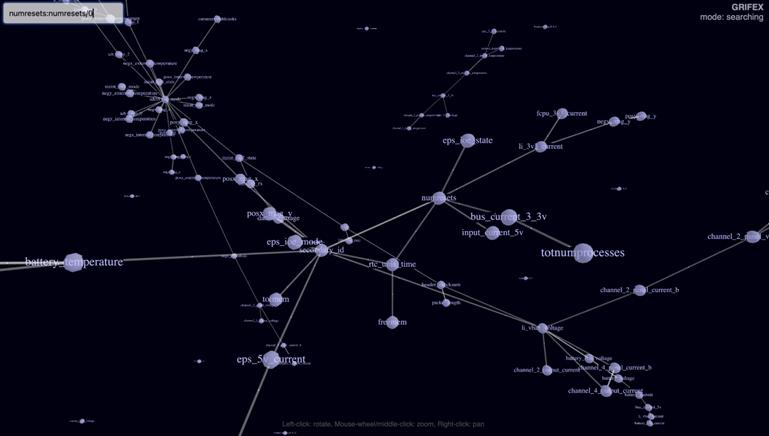
\includegraphics[width=0.80\textwidth]{grifex_graph}\label{fig:grifex_graph}}
        ~\caption{(\ref{fig:grifex_resets_vs_solar_params}) - точечная диаграмма количества принудительных перезагрузок основного процессора с набором параметров активности Солнца для спутника GRIFEX; (\ref{fig:grifex_graph}) - 3D граф связности параметров телеметрии спутника GRIFEX}
        \label{fig:combined_figure}
    \end{figure}

    \begin{figure}[htbp]
        \centering
        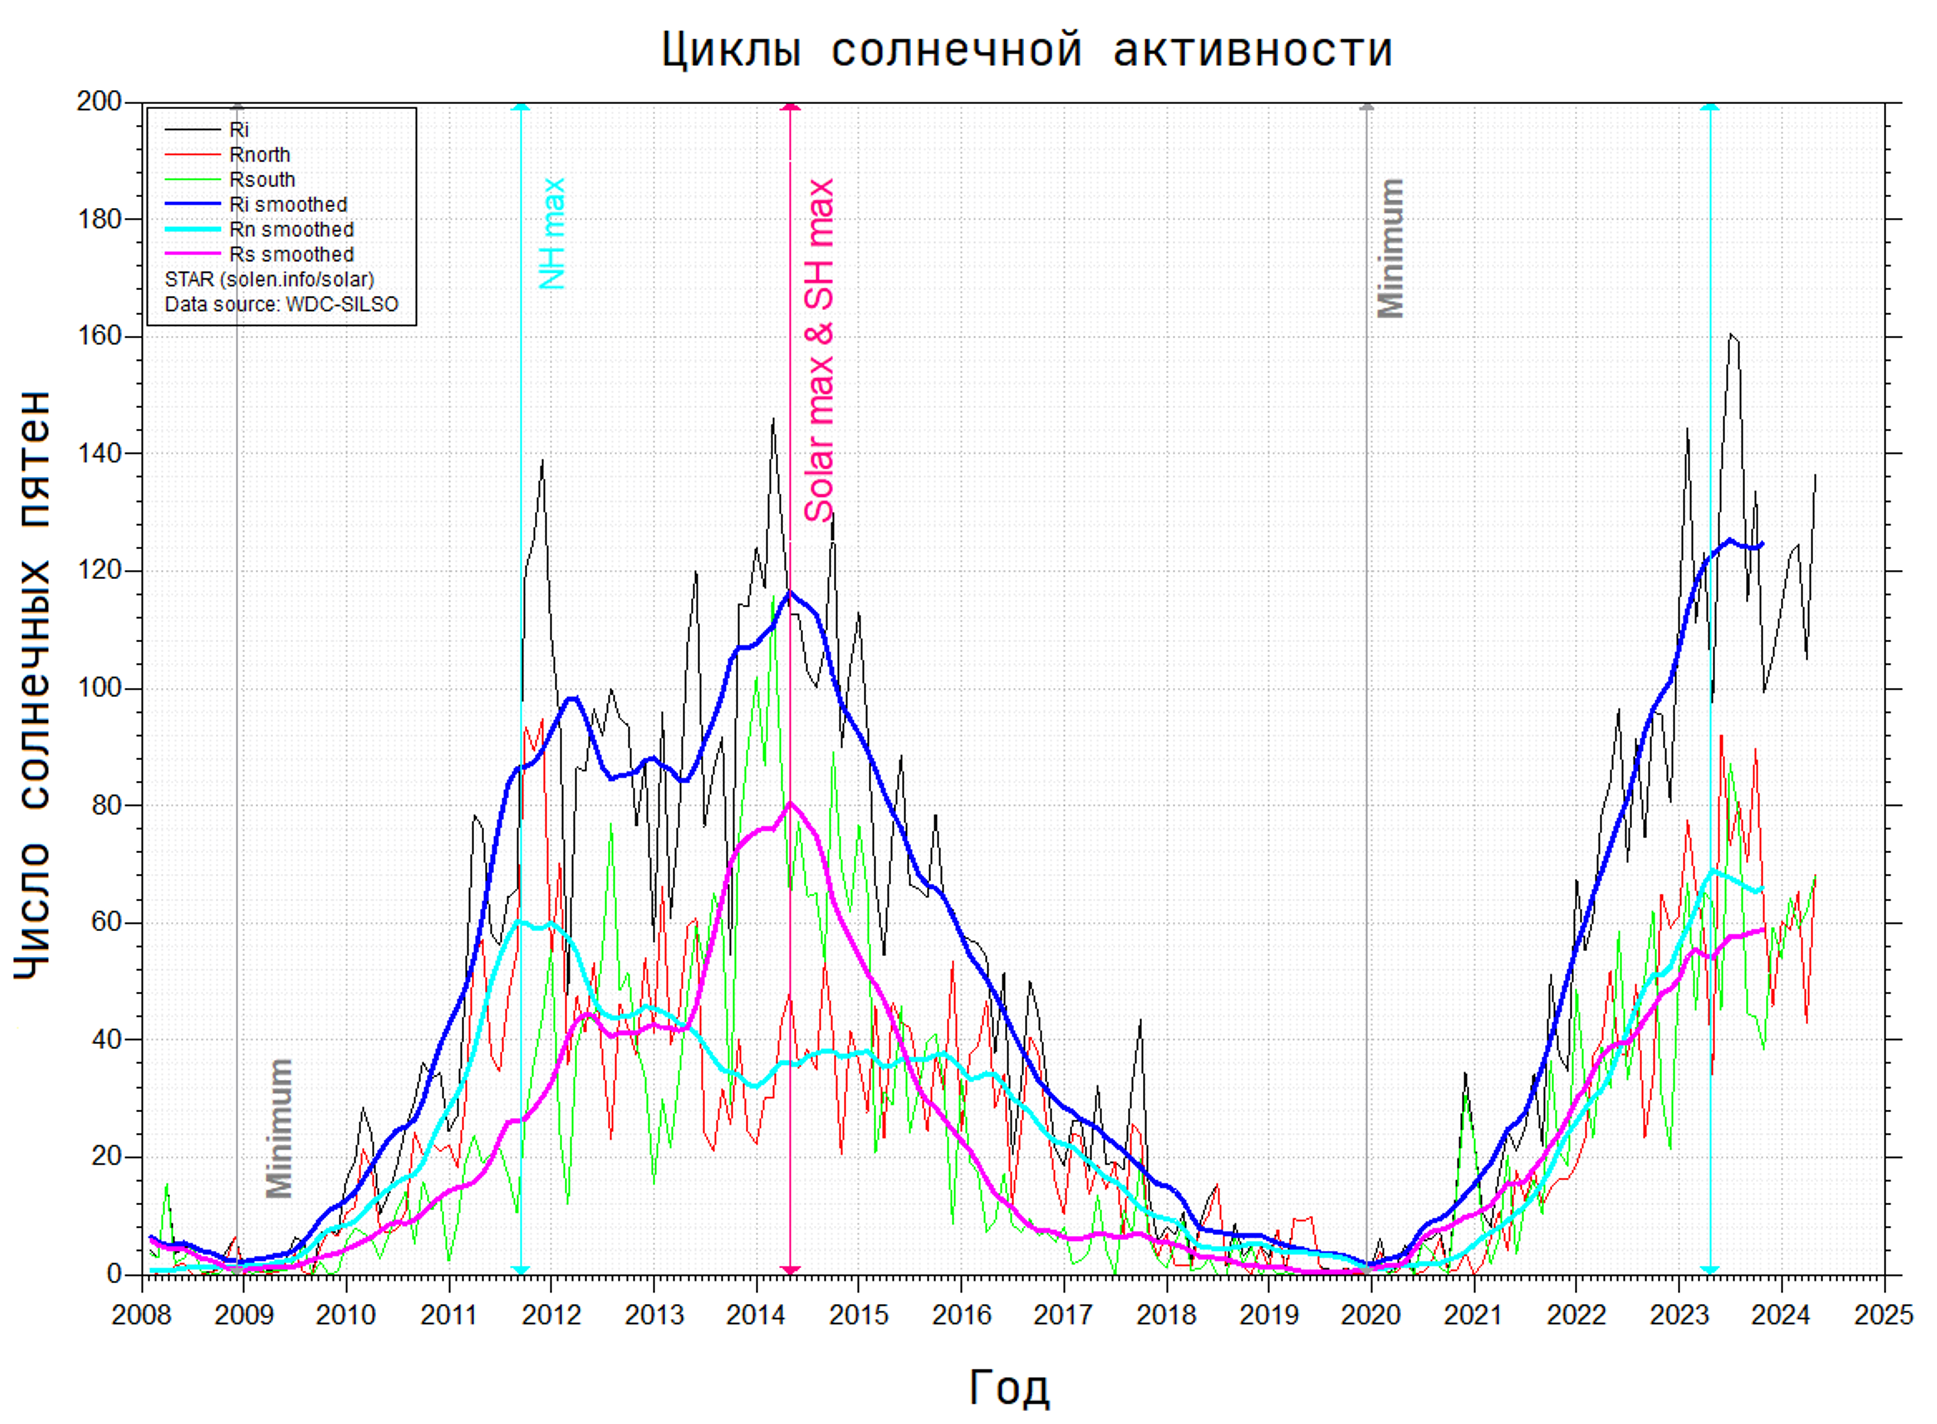
\includegraphics[width=1.0\textwidth]{solar_activity_plot}
        ~\caption{График солнечной активности активности с 2008 по 2024, наблюдаемые значения (источник - NASA SWPC/NOAA)}
        \label{fig:solar_activity_plot}
    \end{figure}

    Как видно, количество перезагрузок основного процессора GRIFEX стремительно накапливалось в период 2019–2020 г., когда индексы солнечной активности SWPC/SWO и f10.7 см были относительно постоянны.
    С 2020 начался новый 5-летний цикл солнечной активности, что соответствуют замедлению роста количества перезагрузок.
    Причина такого поведения объясняется графом связности.
    Из анализа графа видно, все взаимозависимые параметры телеметрии образуют взаимосвязанные ветки относительно времени (rtc\_unix\_time), а также относительно критичных параметров.
    Общее количество перезагрузок основного процессора (numresets) непосредственно связанно с токовым потреблением в бортовой системе питания, в частности, со значением тока на общей шине питания (battery\_bus\_current), с уровнем тока на шине 3.3 В (bus\_current\_3\_3v), с уровнем тока на шине 3.3 В основного процессора (fcpu\_3v3\_current), с уровне тока на шине 3.3 В аккумулятора (li\_3v3\_current).
    Из графа также видно, что на количество перезагрузок процессора влияет число запущенных процессов (totnumprocesses).
    Можно предположить, что количество перезагрузок связанно с просадкой напряжения на шине питания за счет низкой температуры на аккумуляторах (battery\_temperature).
    При увеличении солнечной активности увеличился общий световой поток, что привело к повышению температуры, стабилизации напряжения и несвойственному замедлению роста числа перезагрузок процессора.

    Таким образом, доработанная и адаптированная модель Polaris ML может быть использована для комплексного анализа взаимосвязей и влияния различных факторов на работу бортовой электроники наноспутников, в частности, солнечной активности.
    Оценка большего объема данных позволит выявить наиболее уязвимые системы спутника для разработки безопасных режимов работы его бортового оборудования в условиях агрессивной солнечной активности.

    \subsection{Оценка Эффективности}
    Применение разнообразных методов обнаружения аномалий в Polaris ML позволяет получать более полную картину о состоянии космического аппарата и выявлять широкий спектр потенциальных проблем. Однако, для принятия обоснованных решений необходимо уметь оценивать эффективность выбранных алгоритмов и интерпретировать полученные результаты.
    Polaris ML предоставляет инструменты для оценки качества моделей обнаружения аномалий на основе метрик, таких как:

    \begin{itemize}
        \item Точность (Precision): Доля правильно идентифицированных аномалий среди всех объектов, помеченных как аномалии.
        \item Полнота (Recall): Доля правильно идентифицированных аномалий среди всех реально существующих аномалий в данных.
        \item F1-мера: Гармоническое среднее между точностью и полнотой, является сбалансированной метрикой для оценки общей производительности модели.
    \end{itemize}

    Важно отметить, что не существует универсального метода, идеально подходящего для всех случаев.
    Выбор оптимального метода и интерпретация результатов требует экспертной оценки и учета специфики решаемой задачи.
    Визуализация результатов работы алгоритмов обнаружения аномалий играет важную роль в процессе анализа.
    Polaris ML предоставляет возможность отображать аномалии на графиках, диаграммах и в трехмерном пространстве, что помогает лучше понимать природу обнаруженных отклонений и их связь с другими параметрами телеметрии.

    \subsection{Интерактивный Анализ.}

    Для удобства пользователей Polaris ML предоставляет возможности интерактивного анализа данных.
    Пользователи могут самостоятельно выбирать методы обнаружения аномалий, настраивать их параметры, визуализировать результаты и проводить дополнительные исследования.
    Интерактивный режим работы позволяет экспертам глубже погрузиться в анализ данных, выдвигать гипотезы и проверять их на практике, что способствует более эффективному обнаружению аномалий и выявлению скрытых закономерностей в работе космических систем.

    \subsection{Интеграция с Системой Принятия Решений.}

    Обнаружение аномалий - это только первый шаг на пути к обеспечению надежности и безопасности космических аппаратов.
    Следующим важным этапом является интеграция полученных результатов с системой принятия решений.
    Polaris ML предоставляет возможность экспорта обнаруженных аномалий и связанных с ними данных в различные форматы, что позволяет интегрировать их с другими системами мониторинга и управления космическими аппаратами.
    Например, информация об аномалиях может быть использована для генерации автоматических оповещений для операторов наземного комплекса управления,
    запуска дополнительных диагностических процедур на борту космического аппарата или корректировки плана полета или режимов работы бортовых систем.

    Эффективная интеграция Polaris ML с существующей инфраструктурой управления космическими миссиями позволяет создать единую систему мониторинга и диагностики, способную своевременно выявлять и предотвращать потенциальные проблемы.

    \subsection{Дальнейшие планы по расширению инструментария}

    Помимо XGBoost, Polaris ML может использовать и другие методы выявления аномалий, включая:

    Методы, основанные на расстоянии: Евклидово расстояние, Манхэттенское расстояние, расстояние Махаланобиса.
    Методы, основанные на плотности: Local Outlier Factor (LOF), Isolation Forest.
    Методы машинного обучения: One-Class SVM, автоэнкодеры.

    Выбор конкретных методов зависит от характеристик данных и целей анализа.

    \newpage

    \titleformat{\section}[block]{\large\bfseries\filcenter}{}{0em}{}
    \section{Заключение}

    В ходе данной работы была проведена комплексная оценка влияния космической погоды на работу бортовой электроники космических аппаратов, а также разработана и оптимизирована платформа Polaris ML для анализа больших данных телеметрии.
    Разработка Polaris ML позволила создать более совершенную инфраструктуру для анализа данных, основанную на модели машинного обучения XGBoost. В ходе работы были проведены оптимизация и доработка ядра библиотеки XGBoost, что позволило повысить точность и скорость предсказания аномалий в телеметрии.
    Для проверки эффективности платформы Polaris ML был проведен анализ данных телеметрии космического аппарата GRIFEX. Полученные результаты подтвердили возможность использования Polaris ML для обнаружения и анализа аномалий, связанных с влиянием космической погоды.
    Результаты работы открывают широкие возможности для повышения безопасности и эффективности космических миссий. Развитие Polaris ML позволит создавать интеллектуальные системы поддержки принятия решений, которые способны самостоятельно анализировать данные о состоянии космического аппарата, оценивать риски и предлагать оптимальные варианты действий, тем самым снижая нагрузку на операторов и ускоряя процесс принятия решений.
    В дальнейшем планируется продолжить развитие Polaris ML, добавив новые функции и возможности, такие как автоматическая интерпретация обнаруженных аномалий и расширенный анализ данных с использованием различных моделей машинного обучения. Polaris ML имеет все шансы стать незаменимым инструментом для обеспечения безопасности и эффективности космических миссий будущего.

    \newpage

    \bibliography{main}
    \bibliographystyle{plain}

    \newpage

    \appendix

    \titleformat{\section}[block]{\large\bfseries\filcenter}{}{0em}{}
    \titleformat{\subsection}[block]{\textnormal\bfseries}{}{0em}{}

    \section{Приложения} \label{sec:attachements}

    \subsection{Приложение \arabic{subsection}} \label{subsec:polaris_learn_config}

    Используемая конфигурация для нейронного ансамбля формируемого XGBoost
    
    \begin{verbatim}
        {
        "use_gridsearch": false,
        "random_state": 43,
        "test_size": 0.2,
        "gridsearch_scoring": "neg_mean_squared_error",
        "gridsearch_n_splits": 6,
        "dataset_cleaning_params": {
            "col_max_na_percentage": 100,
            "row_max_na_percentage": 100
            },
        "model_cpu_params": {
            "objective": "reg:squarederror",
            "n_estimators": 81,
            "learning_rate": 0.1,
            "n_jobs": 32,
            "predictor": "cpu_predictor",
            "tree_method": "auto",
            "max_depth": 8
            },
        "model_params": {
            "objective": "reg:squarederror",
            "n_estimators": 80,
            "learning_rate": 0.1,
            "n_jobs": 32,
            "max_depth": 8
            }
        }
    \end{verbatim}

    \subsection{Приложение \arabic{subsection}} \label{subsec:xgboost_cuda_shared_memory_upgrade}
   Примеры улучшений ядра XGBoost на языке CUDA от компании NVIDIA: Следующее ядро использует общую память для лучшей локализации данных.

    \begin{lstlisting}[language=C++, label={lst:xgboost_shared_memory_calculation}]
        // The following kernel utilizes the shared memory for better data locality.
        template <typename Loader, typename Data>
        __global__ void PredictLeafKernelSharedMem(Data data,
                                                  common::Span<const RegTree::Node> d_nodes,
                                                  common::Span<half> d_out_predictions,
                                                  common::Span<size_t const> d_tree_segments,

                                                  common::Span<FeatureType const> d_tree_split_types,
                                                  common::Span<uint32_t const> d_cat_tree_segments,
                                                  common::Span<RegTree::CategoricalSplitMatrix::Segment const> d_cat_node_segments,
                                                  common::Span<uint32_t const> d_categories,

                                                  size_t tree_begin, size_t tree_end, size_t num_features,
                                                  size_t num_rows, size_t entry_start, bool use_shared,
                                                  float missing) {
          const auto ridx = blockDim.x * blockIdx.x + threadIdx.x;
          if (ridx >= num_rows) {
            return;
          }

          // Allocate shared memory for data, adjust based on your data structure.
          // For example, this assumes a 2D array for data.
          __shared__ float shared_data[BLOCK_SIZE * NUM_FEATURES];

          // Load data into shared memory
          if (threadIdx.x < num_features) {
            shared_data[threadIdx.x] = data[ridx * num_features + threadIdx.x];
          }
          __syncthreads();

          Loader loader(shared_data, use_shared, num_features, num_rows, entry_start, missing);

          for (size_t tree_idx = tree_begin; tree_idx < tree_end; ++tree_idx) {
            TreeView d_tree{
                tree_begin,          tree_idx,           d_nodes,
                d_tree_segments,     d_tree_split_types, d_cat_tree_segments,
                d_cat_node_segments, d_categories};

            bst_node_t leaf = -1;

            if (d_tree.HasCategoricalSplit()) {
              leaf = GetLeafIndex<true, true>(ridx, d_tree, &loader);
            } else {
              leaf = GetLeafIndex<true, false>(ridx, d_tree, &loader);
            }

            d_out_predictions[ridx * (tree_end - tree_begin) + tree_idx] = __float2half_rn(leaf);
          }
        }
    \end{lstlisting}

    \subsection{Приложение \arabic{subsection}} \label{subsec:xgboost_cuda_tensor_upgrade}
    Примеры улучшений ядра XGBoost на языке CUDA от компании NVIDIA: используются тензорные ядра для умножения матриц, предполагается, что входные данные представлены в матричной форме.

    \begin{lstlisting}[language=C++, label={lst:xgboost_tensor_kernel_calculation}]
        template <typename Loader, typename Data>
        __global__ void PredictLeafKernelTensorCore(Data data,
                                                  common::Span<const RegTree::Node> d_nodes,
                                                  common::Span<half> d_out_predictions,
                                                  common::Span<size_t const> d_tree_segments,

                                                  common::Span<FeatureType const> d_tree_split_types,
                                                  common::Span<uint32_t const> d_cat_tree_segments,
                                                  common::Span<RegTree::CategoricalSplitMatrix::Segment const> d_cat_node_segments,
                                                  common::Span<uint32_t const> d_categories,

                                                  size_t tree_begin, size_t tree_end, size_t num_features,
                                                  size_t num_rows, size_t entry_start, bool use_shared,
                                                  float missing) {
          const auto ridx = blockDim.x * blockIdx.x + threadIdx.x;
          if (ridx >= num_rows) {
            return;
          }

          // Assume data is organized in a matrix, for example,
          // [num_rows x num_features].

          // Declare cuBLAS handles
          cublasHandle_t handle;
          cublasCreate(&handle);

          // Allocate device memory for matrices
          half* d_matrixA;
          half* d_matrixB;
          half* d_matrixC;
          size_t size = num_rows * num_features * sizeof(half);
          cudaMalloc(&d_matrixA, size);
          cudaMalloc(&d_matrixB, size);
          cudaMalloc(&d_matrixC, size);

          // Copy data to device memory (adjust based on your data organization)
          cudaMemcpy(d_matrixA, data, size, cudaMemcpyHostToDevice);

          // Initialize d_matrixB (assuming a diagonal matrix with values of 1.0f)
          for (size_t i = 0; i < num_features; ++i) {
            d_matrixB[i * num_features + i] = __float2half_rn(1.0f);
          }

          // Perform matrix multiplication using cuBLAS
          cublasSgemm(handle, CUBLAS_OP_N, CUBLAS_OP_N,
                      num_rows, num_features, num_features,
                      &__float2half_rn(1.0f), d_matrixA, num_features,
                      d_matrixB, num_features,
                      &__float2half_rn(0.0f), d_matrixC, num_features);

          // Free device memory
          cudaFree(d_matrixA);
          cudaFree(d_matrixB);
          cudaFree(d_matrixC);

          // Destroy cuBLAS handle
          cublasDestroy(handle);

          Loader loader(data, use_shared, num_features, num_rows, entry_start, missing);

          for (size_t tree_idx = tree_begin; tree_idx < tree_end; ++tree_idx) {
            TreeView d_tree{
                tree_begin,          tree_idx,           d_nodes,
                d_tree_segments,     d_tree_split_types, d_cat_tree_segments,
                d_cat_node_segments, d_categories};

            bst_node_t leaf = -1;

            if (d_tree.HasCategoricalSplit()) {
              leaf = GetLeafIndex<true, true>(ridx, d_tree, &loader);
            } else {
              leaf = GetLeafIndex<true, false>(ridx, d_tree, &loader);
            }

            d_out_predictions[ridx * (tree_end - tree_begin) + tree_idx] = __float2half_rn(leaf);
          }
        }
    \end{lstlisting}

    \subsection{Приложение \arabic{subsection}} \label{subsec:dot_diagram_code}
    Код на языке программирования python предназначенный для построения точечных диаграм извлеченных нормализованных данных.

    \begin{lstlisting}[language=python, label={lst:dot_diagram_code}]
        with open(satellite_json, 'r') as file:
            json_stream: str = file.read()

        json_data: dict = json.loads(json_stream)

        if not json_data:
            logger.error("Json data is empty")
            exit(1)


        class Satellite:
            def __init__(self, norad_id: int, name: str, observations_amount: int):
                self.norad_id: int = norad_id
                self.name: str = name
                self.observations_amount: int = observations_amount


        metadata: dict = json_data['metadata']

        satellite: Satellite = Satellite(
            metadata['satellite_norad'],
            metadata['satellite_name'],
            metadata['total_frames']
        )

        solar_and_satellite_parameters_names: Dict[str, str] = metadata['analysis'][
            'column_tags']

        solar_parameters_names: List[str] = metadata['analysis']['feature_columns']

        satellite_parameters_names: List[str] = [value for value in
                                                 solar_and_satellite_parameters_names if
                                                 value not in solar_parameters_names]

        frames: dict = json_data['frames']

        allowed_types: Union = Union[int, float, bool, str]

        observation_data: List[Dict[str, Timestamp]] = []

        # 'time' is unix timestamps, convertor - https://www.epochconverter.com/
        for frame in frames:
            observation_time = pd.to_datetime(frame['time'])
            fields: Dict[Any, Any] = {key: value['value'] for key, value in
                                      frame['fields'].items() if
                                      isinstance(value, dict)}
            observation_data.append({'time': observation_time, **fields})

        observation_dataframe: pd.DataFrame = pd.DataFrame(observation_data).set_index(
            'time').dropna().select_dtypes(include=np.number)

        observation_dataframe = observation_dataframe.loc[:,
                                observation_dataframe.nunique() > 1]  # Select columns with more than 1 unique value
    \end{lstlisting}
    
\end{document}
